\chapter{Supersymmetry and the Standard Model}
\label{ch:SUSY}

The fundamental theory of particle physics, known as the Standard Model (SM) can predict precise interactions between the fundamental particles in our universe. With these predictions we can confirm processes, but there are some aspects of the universe that have not yet been explained. In this Chapter, we will analyze the Standard Model, look at some specific shortcomings, and introduce supersymmetry as a possible solution.

\section{The Standard Model}
\label{sec:SM}

After decades of theoretical and experimental research the SM has been developed into a theory that explains the Electromagnetic (EM), Strong, and Weak forces. The SM has not yet been able to include Gravity within the theory. With the robust theoretical and experimental methods used in the SM, we have discovered new elementary particles and predicted others. 

\subsection{The Fundamental Particles}

 All visable matter can be explained by three kinds of elementary particles: leptons, quarks, and gauge bosons. Each of these can be distinguished by various quantum properties. The leptons and quarks are fermions, which are particles that have half-integer spin. Leptons are particles that only interact with the EM and Weak force, while quarks interact with all three forces of the SM. The gauge bosons are the force carries for each respective force and have integer spin. 
 
 There are three generations of leptons and quarks which are differentiated by a charge $\pm e$, the charge of an electron. Leptons have three different charged particles: electron $(e)$, muon $(\mu)$, and tau $(\tau)$, with each charged particle having a corresponding neutrino $(\nu)$ of the same flavor, see fig \ref{SMParticles}. Quarks are also separated into three generations of doublets, the down-type $(-\frac{1}{3}e)$: down $(d)$, strange $(s)$, and bottom $(b)$ and up-type $(\frac{2}{3}e)$: up $(u)$, charm $(c)$, and top $(t)$, see fig \ref{SMParticles}. Each of the quarks has a color associated with it which is analogous to an electric charge, except there are three colors charges: red, blue, and green.  

\begin{figure}
 	\centering
	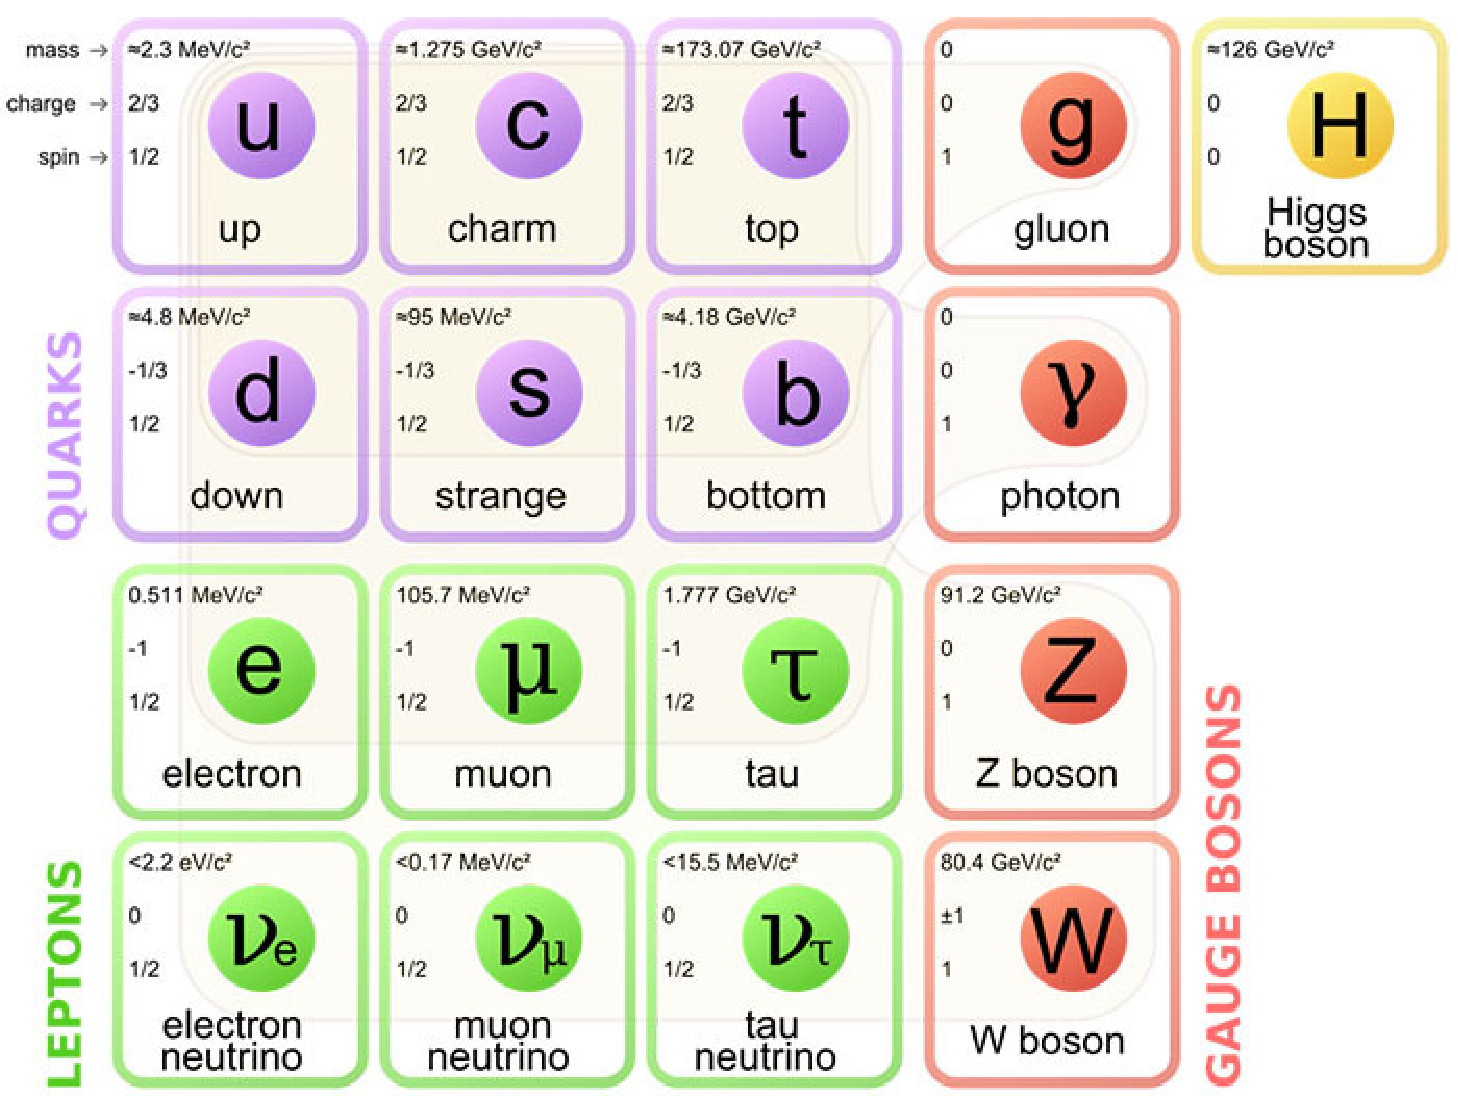
\includegraphics[width=0.75\textwidth]{StandardModel.pdf}
 	\caption[Standard Model particles]{The fundamental particles of the Standard Model. There are three generations of quarks and leptons. Along with the five bosons, where four of them relate to the interactions of the three forces included in the SM: Electromagnetism, the Weak force, and the Strong force and the final being the Higgs boson.}
 	\label{SMParticles} 
\end{figure}
 
 \subsection{Quantum Field Theory}
 \label{QFT}
 
 The interactions of all these particles are described by quantized fields whose operators describe the creation and annihilation of particles. Each of the fields of the SM have a corresponding gauge boson, see fig. \ref{SMParticles}. The most well-known being the EM field and its interactions. In order to write a concise theory of the particles in the SM, the symmetry and conservation laws of the SM can be derived by starting with Noether's Theorem.
 
 \subsection{Noether's Theorem}
 
 Noether's theorem states,"to each symmetry of a local Lagrangian, there corresponds a conserved current". This can be done by allowing for an infinitesimal symmetry variation. Requiring the Lagrangian to be invariant under $\phi(x)\rightarrow\phi^\prime(x)=\phi(x)+\alpha\Delta\phi(x)$, where $\alpha$ is infinitesimal real parameter and $\Delta\phi$ is a deformation to the field, up to a 4-divergance, the Lagrangian transforms as,
 \begin{equation}\label{LagrangeFluctuation}
 \mathcal{L}(x)\rightarrow\mathcal{L}(x)+\alpha\partial_\mu\mathcal{J}^\mu(x),
 \end{equation}
 where $\mathcal{J}^\mu$ is a current. If we apply the Euler-Lagrange equation,
 \begin{equation}
 \partial_\mu(\frac{\partial\mathcal{L}}{\partial(\partial_\mu\phi)})-\frac{\partial\mathcal{L}}{\partial\phi}=0,
 \end{equation}
 to Eqn. \ref{LagrangeFluctuation} with the addition of the fluctuation of the particle field. After some simplification we get a conserved current \cite{halzen_quarks_1984, peskin_introduction_1995},
 \begin{equation}
 \begin{split}
 \partial_\mu j^\mu(x)&=0, \text{ where}\\
 j^\mu(x)&=\frac{\partial\mathcal{L}}{\partial(\partial_\mu\phi)}\Delta\phi-\mathcal{J}^\mu
 \end{split}.
 \end{equation} We see from the above equation that the current $j^\mu(x)$ of the Lagrangian is conserved. Now let's apply this to the particle fields of the SM.
 
 \subsection{Quantum Electrodynamics (QED)}
 
 First, we start with the assumption that the wave function $\psi(x)$ should transform as,
 \begin{equation}\label{U1gauge}
 \psi(x)\rightarrow e^{i\alpha(x)}\psi(x),
 \end{equation}
 where $\alpha(x)$ has an arbitrary dependence on space and time. 
 If one were to include this into the Lagrangian for a spin-$1/2$ particle in a vacuum,
 \begin{equation}\label{DiracLag}
\mathcal{L}_{QED}^{vac}=i\overline{\psi}\gamma^\mu\partial_\mu\psi-m\overline{\psi}\psi
\end{equation}
 where the $\gamma^\mu$ are the Dirac matrices, $\partial_\mu$ is the partial derivative, $\overline{\psi}$ is the hermitian conjugate of the wavefuntion $\psi$, and $m$ is the mass of the particle. As a small aside, the bilinear quantities $\overline{\psi}(4\times4)\psi$ have certain properties under lorentz transformations when the $4\times4$ matix is a $\gamma$-matrices. These are of the form,
\begin{equation} \label{gammaMatrix}
\gamma^0=
\begin{bmatrix}
\boldsymbol{I} & 0 \\
0 & -\boldsymbol{I}
\end{bmatrix},
\boldsymbol{\gamma}=
\begin{bmatrix}
0 & \boldsymbol{\sigma} \\
-\boldsymbol{\sigma} & 0
\end{bmatrix},
\gamma^5=
\begin{bmatrix}
0 & \boldsymbol{I} \\
\boldsymbol{I} & 0
\end{bmatrix}
\end{equation}
where the $\boldsymbol{I}$ is the identity matrix and $\boldsymbol{\sigma}$ are the Dirac matrices. We can combine the first two parts of Eqn. \ref{gammaMatrix} and write it compactly as $\gamma^\mu$ where $\mu=0,1,2, \text{and }3$. The possible interesting quantities of the above transformations are shown in Table \ref{Transformations}.

\begin{table}
\centering
\begin{tabular}{|c|c|c|c|}
\hline
Type & Form & Components & Space Inversion \\
\hline
\hline
 Scalar &  $\overline{\psi}\psi$ &  1 & $+$ under $P$ \\
 Vector & $\overline{\psi}\gamma^\mu\psi$ & 4 & Space compts.: $-$ under $P$ \\
 Tensor & $\overline{\psi}\sigma^{\mu\nu}\psi$ & 6 &  \\
 Axial Vector & $\overline{\psi}\gamma^5\gamma^\mu\psi$ & 4 & Space compts.: $+$ under $P$ \\
 Pseudoscalar & $\overline{\psi}\gamma^5\psi$ & 1 & $-$ under $P$ \\
 \hline
\end{tabular}
\caption[Fermion Currents]{A table showing all forms of the fermion currents. These can be symmetric under parity transformation in all or some components.}
\label{Transformations}
\end{table}

To allow for the field to be invariant, we must include a derivative, $D_\mu$, that is covariant under phase transformations,
 \begin{equation}\label{QEDCovariantD}
 D_\mu\equiv\partial_\mu-ieA_\mu.
 \end{equation}
 The covariant derivative includes the vector field $A_\mu$ which must also transform as,
  \begin{equation}\label{PhotonField}
 A_\mu\rightarrow A_\mu+\frac{1}{e}\partial_\mu\alpha.
 \end{equation}
 So after requiring that there be a local gauge transformation, we were forced to introduce a vector field $A_\mu$, called the gauge field, which couples to Dirac particles in the same way as the photon field. We will think of this new field as the real photon field, which means we need to add a kinematic energy portion to the lagrangian. This kinematic term will be invariant under Eqn. \ref{PhotonField}, which leads us to final representation of the QED lagrangian which can be written down concisely as, 
\begin{equation}\label{LagrangianQED}
\mathcal{L}_{QED}=\overline{\psi}(i\gamma^\mu\partial_\mu-m)\psi+e\overline{\psi}\gamma^{\mu}A_{\mu}\psi-\frac{1}{4}F^{\mu\nu}F_{\mu\nu},
\end{equation}
where $A_{\mu}$ is the EM field operator and $F^{\mu\nu}$ is the EM field tensor. This Lagrangian describes the interactions between spin-$1/2$ charged particles and the $U(1)$ EM force. Each of the parts of this equation are lorentz invariant which allows this to be true in all reference frames. 

\begin{figure}
 	\centering
	\includegraphics[width=0.75\textwidth]{QEDRules.png}
 	\caption[QED Feynman Diagrams]{The possible feynman diagrams in QED. The $e$ can be replaced with any spin-$1/2$ charged particle. We see that the electron and photon can propagate freely in space or a vertex with one photon and a particle-antiparticle pair is allowed.}
 	\label{QEDRules} 
\end{figure}

From the QED Lagrangian Eqn. \ref{LagrangianQED}, we see that particles that interact electromagnetically can interact with the photon. This can be shown as a feynman diagram, see Fig. \ref{QEDRules}, which has a vertex interaction with a photon and a particle-antiparticle pair. These, and the inclusion of freely moving particles, are the basic types of feynman diagrams for QED. 

\subsection{Quantum Chromodynamics}

Let's now transition from the description of the $U(1)$ EM field to the $SU(3)$ Quantum Chromodynamic (QCD) field and the transformation of quark fields. A quark in a vaccuum is described by,
\begin{equation}\label{LagrangianQCDVacuum}
\mathcal{L}_{QCD}^{vac}=\overline{q}_j(i\gamma^\mu\partial\mu-m)q_j,
\end{equation}
where $q_1, q_2,$ and $q_3$ are the three color fields. From this we want to require that the field is again invariant under another local phase transformation such as,
\begin{equation}
q(x)\rightarrow Uq(x)\equiv e^{i\alpha_a(x)T_a}q(x),
\end{equation}
where $U$ is a $3\times3$ unitary matix, $T_a$ with $a=1,\ldots,8$ are a set of linearly independent traceless $3\times3$ matrices, and $\alpha_a$ are the group parameters. Since the generators $T_a$ do not necessarily commute with each other, we can see that it is a non-Abelian transformation and the commutator can be represented as,
\begin{equation}
[T_a, T_b]=if_{abc}T_c,
\end{equation}
where $f_{abc}$ are constants. 

We need to impose $SU(3)$ local gauge invariance on Eqn. \ref{LagrangianQCDVacuum}, to allow for the following phase transformations,
\begin{equation}
\begin{split}
& q(x)\rightarrow(1+i\alpha_a(x)T_a)q(x), \\
& \partial_\mu q\rightarrow(1+i\alpha_aT_a)\partial_\mu q+iT_aq\partial_\mu\alpha_a.
\end{split}
\end{equation}
From this is seems straight forward that we can proceed in exactly the same manner as QED, which is to add a transformation to the derivative,
\begin{equation}
D_\mu=\partial_\mu+ig_Q T_aG_\mu^a.
\end{equation}
where the field $G_\mu^a$ transforms as, 
\begin{equation}
G_\mu^a\rightarrow G_\mu^a-\frac{1}{g_Q}\partial_\mu\alpha_a,
\end{equation}
where $g_Q$ is the coupling strength of QCD interactions. This will give us a similar Lagrangian to the QED one described above, but this is not sufficient for a non-Abelian gauge transformation and it does not produce a gauge-invariant Lagrangian. One final transformation is required for the $G_\mu^a$ fields, 
\begin{equation}\label{QCDGaugeTransform}
G_\mu^a\rightarrow G_\mu^a-\frac{1}{g_Q}\partial_\mu\alpha_a-f_{abc}\alpha_b G_\mu^c.
\end{equation}

\begin{figure}[!htb]
	\minipage{0.4\textwidth}
	  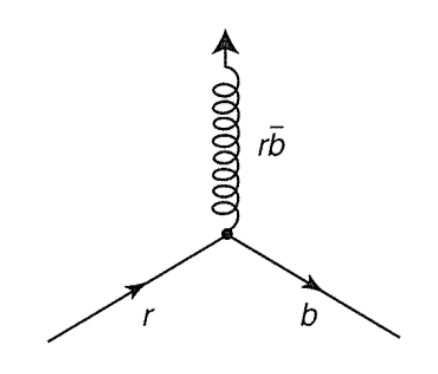
\includegraphics[width=\linewidth]{QCDQuarkRules.png}
	\endminipage\hfill
	\minipage{0.5\textwidth}
	  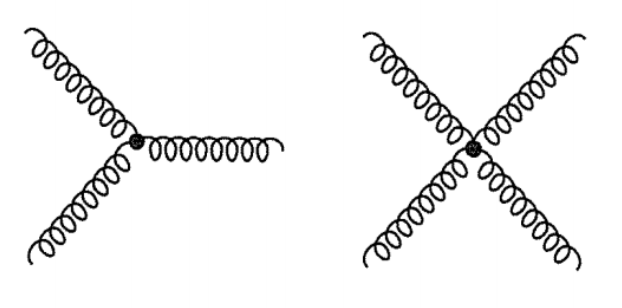
\includegraphics[width=\linewidth]{QCDGluonRules.png}
	\endminipage\hfill
	\caption[QCD Feynman Diagrams]{The possible feynman diagrams in QCD. Each vertex needs to be color neutral. Here is just an example of a red-blue vertex. QCD also includes a 3- and 4-vertex with gluons.}
 	\label{QCDRules} 
\end{figure}

This finally gives us a gauge invariant kinetic energy term for all the $G_\mu^a$ fields and thus we can write the QCD interactions as,
\begin{equation}\label{LagrangianQCD}
\mathcal{L}_{QCD}=\overline{q}(i\gamma^\mu\partial_\mu-m)q-g_Q(\overline{q}\gamma^\mu T_a q)G^a_\mu-\frac{1}{4}G^a_{\mu\nu}G_a^{\mu\nu}.
\end{equation}
From the QCD Lagrangian Eqn. \ref{LagrangianQCD}, we can see that it includes all of the same interactions we showed for QED, but must be color neutral. However, QCD also included a 3- and 4-vertex interaction between the gluons, which arises due to the non-abelian nature of the force. From this, it is easy to tell that QCD is a much more complicated theory. We seem to be missing a vital part of the SM, specifically a theory for the Weakly interacting processes which is mediated by the massive bosons, \W{} and \Z{} from fig. \ref{SMParticles}. 

\subsection{Weak Force}
\label{WeakForce}

The Weak force is responsible for nuclear decay. The Weak force has an interaction of the type $\frac{1}{2}\gamma^\mu(1-\gamma^5)$ so it is a V-A interaction with $SU(2)$ symmetry. From this, we can conclude that it violates Parity. Parity is a transformation from $(x, y, z)\rightarrow(-x,-y,-z)$ or space inversion. Since it violates Parity, the next step is to consider a conservation of $CP$, where $C$ is charge conjugation (particle-to-antiparticle). 

The main experimental implications of this proposed conservation comes from the decay of the neutral Kaon, $K^0(\overline{s}d) \text{ and } \overline{K}^0(s\overline{d})$. These have two $CP$ states which are, $CP\ket{K^0}=-\ket{\overline{K}^0},$ and $CP\ket{\overline{K}^0}=-\ket{K^0}$. Once we normalize these eigenstates of $CP$ we get the corresponding wavefunctions,
\begin{equation}\label{KaonEigenstate}
\ket{K_1}=\left(\frac{1}{\sqrt{2}}\right)(\ket{K^0}-\ket{\overline{K}^0}) \text{ and } \ket{K_2}=\left(\frac{1}{\sqrt{2}}\right)(\ket{K^0}+\ket{\overline{K}^0}),
\end{equation}
where each has the invariance $CP\ket{K_1}=\ket{K_1}$ and $CP\ket{K_2}=-\ket{K_2}$. The two Kaon states are expected to decay into either two pions or three pions for $\ket{K_1}$ and $\ket{K_2}$, respectively. Since there is a greater energy release in the $\ket{K_1}$ state the lifetime of that particle is thought to be less than $\ket{K_2}$. After experimenting on the purity of Kaon decays after a long distance away from an interaction point, we have found that it is possible for the $\ket{K_1}$ to decay into three pions. This is direct evidence of Weak decays violating $CP$ conservation. 

Now the Weak force is mediated by two vector bosons, \W{} and \Z, see fig. \ref{SMParticles}. These are unlike the other forces because these vector bosons have a large mass of $m_\W=80.379\pm0.012$ GeV and $m_Z=91.1876\pm0.0021$ GeV. The \W{} boson is a charged particle and interacts with many nuclear decays. 

\begin{figure}
 	\centering
	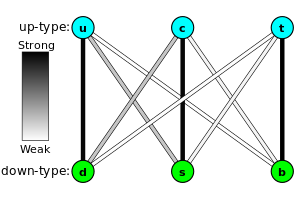
\includegraphics[width=0.5\textwidth]{Quark_weak_interactions.png}
 	\caption[CKM Matrix Couplings]{A gramatical representation to show the couplings for Weak interactions, known as the Cabibbo-Kobayashi-Maskawa Matrix. }
 	\label{CKMInteractions} 
\end{figure}

The \W{} boson interacts very interestingly for quarks in the SM. There is a mixing of flavors of quarks for particles. They will mix partners between up-type and down-type particles, see fig. \ref{CKMInteractions}. [Kobayashi, M. and Maskawa, K. (1973) Progress in Theoretical Physics, 49, 652]. The interactions for the generalized three generations of quarks is known as the Cabibbo-Kobayashi-Maskawa (CKM) matrix,
\begin{equation}\label{CKM}
\begin{bmatrix}
d' \\
s' \\
b' \\
\end{bmatrix} =
\begin{bmatrix}
V_{ud} & V_{us} & V_{ub} \\
V_{cd} & V_{cs} & V_{cb} \\
V_{td} & V_{ts} & V_{tb} \\
\end{bmatrix}
\begin{bmatrix}
d \\
s \\
b \\
\end{bmatrix},
\end{equation}
where for example, $V_{ud}$ is the coupling of $u$ to $d$ which is exactly $(d\rightarrow u+\W^-)$. This matrix can be reduced to a form which has three generalized Cabibbo angles $(\theta_{12},\theta_{23},\theta_{13})$ and a phase factor $(\delta)$. The coupling between the third generation does not mix with the other two generations. From that we can recover the Cabibbo-GIM matrix[cite here]. For the moment, we can only determine these values from experimentation. 

\begin{figure}[!htb]
	\minipage{0.4\textwidth}
	  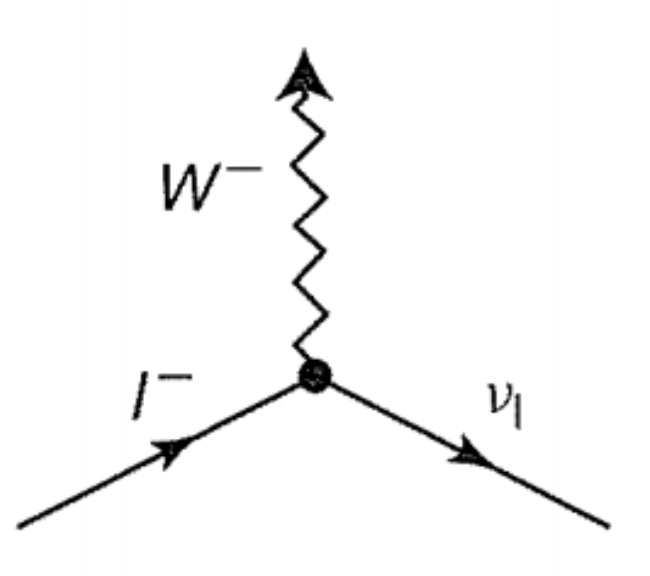
\includegraphics[width=\linewidth]{Wboson_interactions.png}
	\endminipage\hfill
	\minipage{0.4\textwidth}
	  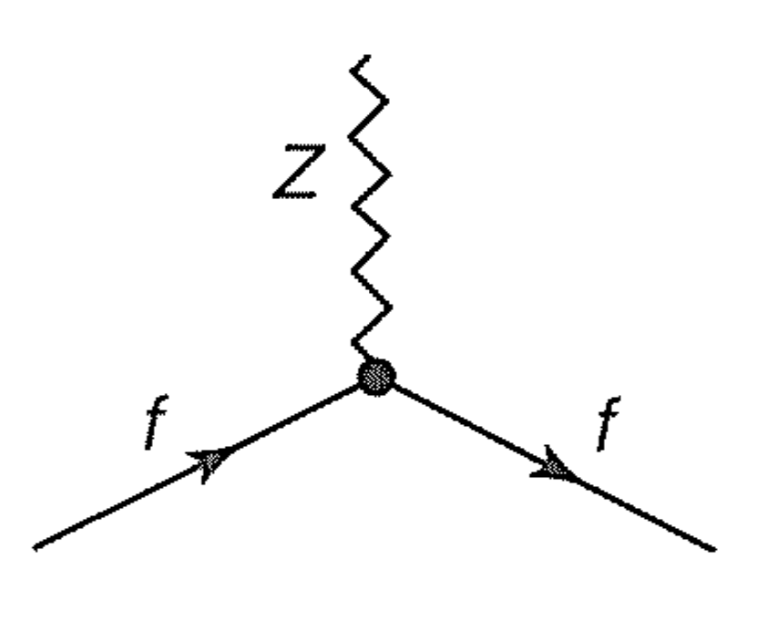
\includegraphics[width=\linewidth]{Zboson_interaction.png}
	\endminipage\hfill
	\caption[Weak Feynman Diagrams]{Feynman diagram for Neutral Weak interaction and the charged weak current.}
 	\label{WeakRules} 
\end{figure}

The \Z{} boson is known as the neutral current. This boson mediates forces between particles and their respective antiparticles, see fig. \ref{ZbosonInteraction}. This interaction for the neutral weak force is $\gamma^\mu(c_V^f-c_A^f\gamma^5)$ which is quite similar to the charged weak interaction, but differs by the constants $c_V^f$ and $c_A^f$. The Weak interactions are shown in Fig. \ref{WeakRules}. We see the charged \W{} boson interactions with the charged leptons and their respective neutrinoes or allows for flavor changing interactions with quarks. The neutral \Z{} boson interacts in the same way as the photon. 

\subsection{The Electroweak Lagrangian}

The simplest group for the Electroweak interaction is $SU(2)_L\times U(1)_Y$ which will give the left-handed interactions in doublets with the addition of massive gauge bosons \W{} and \Z{} with a massless photon. We first consider the free Lagrangian,
\begin{equation}\label{WeakL}
\mathcal{L}=\overline{\psi}_j\gamma^\mu\psi_j,
\end{equation}
where $j$ is the fermion wavefunction. We are not including the mass parameter because it would cause the left and right-handed parts to mix.  This is assumed to transform under the global invariant
\begin{equation}\label{WeakGlobal}
\begin{split}
\chi_L\rightarrow\chi'_L&=e^{i\frac{\tau_a}{2}\alpha^a(x)+i\beta(x)Y}\chi_L, \\
\psi_R\rightarrow\psi'_R&=e^{i\beta(x)Y}\psi_R
\end{split}
\end{equation}
where the transformation $e^{i\frac{\tau_a}{2}\alpha^a(x)}$ with $a = 1, 2, 3$ is the $SU(2)_L$ transformation and only acts on the left-handed doublet. The next step is to require that the Lagrangian is invariant under local $SU(2)_L\times U(1)_Y$. We allow for the following covariant derivatives,
\begin{equation}
\begin{split}
D_\mu\psi_1&=[\partial_\mu-ig_W\frac{\tau_a}{2}W_\mu^a-ig_W^\prime y_1 B_\mu]\psi_1 \\
D_\mu\psi_2&=[\partial_\mu-ig_W^\prime y_2 B_\mu]\psi_2 \\
D_\mu\psi_3&=[\partial_\mu-ig_W^\prime y_3 B_\mu]\psi_3 \\
\end{split}
\end{equation}
where $g_W$ and $g_W^{\prime}$ are the Weak force coupling constants while $W_\mu^a$ and $B_\mu$ are four gauge bosons and can be the possible candidates for $\W^\pm$, \Z and $\gamma$. 

 Just like the above descriptions the fields need to transform along with the wavefuntions and derivatives. These transformations are,
\begin{equation}
\begin{split}
B_\mu\rightarrow&B^\prime_\mu=B_\mu+\frac{1}{g_W^\prime}\partial_\mu\beta(x) \\
W\mu\rightarrow&W^\prime_\mu=U_L W_\mu U^\dagger_L-\frac{1}{g_W}\partial_\mu U_L U_L^\dagger \\
\end{split}
\end{equation}
where $U_L=e^{i\frac{\tau_a}{2}\alpha^a(x)}$. These transformation are similar to the QED and QCD transformation. If we include all of these invariant transformations in the free Weak Lagrangian Eqn. \ref{WeakL} and we get a free invariant Lagrangian, but this does not allow us to include a mass term for the fermions. Therefore this is not a viable procedure to include the Electroweak interactions into the model. In order to do this we must include the Higgs Mechanism.

\subsection{The Higgs Mechanism}\label{HiggsMechanism}

We are interested in the spontaneous symmetry breaking of a local $SU(2)$ group. Specifically, the following Lagrangian,
\begin{equation}\label{HiggsLagrangian}
\mathcal{L}=(\partial_\mu\phi)^\dagger(\partial^\mu\phi)-\mu^2\phi^\dagger\phi-\lambda(\phi^\dagger\phi)^2,
\end{equation}
with $\phi$ being a $SU(2)$ doublet of complex scalar fields,
\begin{equation}
\phi=\frac{1}{2}
\begin{bmatrix}
\phi_1+i\phi_2 \\
\phi_3+i\phi_4
\end{bmatrix}
\end{equation} 
and is invariant under global $SU(2)$ phase transformations $\phi\rightarrow e^{i\alpha_a\tau_a/2}\phi$. To allow for local invariance, we first allow for a covariant derivative,
\begin{equation}
D_\mu=\partial_\mu+ig_W \frac{\tau_a}{2}W_\mu^a,
\end{equation}
where we now have three gauge fields, $W_\mu^a$. If we assume an infanitesimal gauge transformation for the $SU(2)$ doublet $\phi(x)\rightarrow\phi'(x)=(1 +i\frac{\tau_a}{2}\alpha^a(x))\phi(x)$, then the gauge fields will transform as,
\begin{equation}\label{HiggVectorTransform}
W^a_\mu\rightarrow W^a_\mu-\frac{1}{g_W}\partial_\mu\alpha_a-f_{abc}\alpha_bW^c_\mu.
\end{equation}

You can see that Eqn. \ref{HiggVectorTransform} is similar to Eqn. \ref{QCDGaugeTransform} where we have replaced the QCD gauge field with the three gauge fields $W_\mu^a$. If we include these locally invariant transformations into the above $SU(2)$ Lagrangian we get,
\begin{equation}\label{WeakLagrangian}
\mathcal{L}=(\partial_\mu\phi+ig_W\frac{1}{2}\tau_{a}W^{a}_\mu\phi)^\dagger(\partial^\mu\phi+ig_W\frac{1}{2}\tau_{a}W^{a\mu}\phi)-\mu^2\phi^\dagger\phi+\lambda(\phi^\dagger\phi)^2-\frac{1}{4}W^{a}_{\mu\nu}W^{a\mu\nu},
\end{equation}
where the gauge field kinetic term has been included at the end. The most interesting regions of this Lagrangian is when $\mu^2<0$ and $\lambda>0$, and the potential has a minimum at $\phi^\dagger\phi=-\frac{\mu^2}{2\lambda}$. With this we will expand the potential around the minimum and require that,
\begin{equation}
\phi_1=\phi_2=\phi_4=0, \phi_3^2=-\frac{\mu^2}{2\lambda}\equiv v^2.
\end{equation}
This is the spontaneous symmetry breaking of the $SU(2)$ symmetry, because of this we are able to substitute an expansion for the field,
\begin{equation}
\phi=\sqrt{\frac{1}{2}}
\begin{bmatrix}
0 \\
v+h(x)
\end{bmatrix}
\end{equation}
with this specific transformation of the $SU(2)$ doublet and the simplification of Eqn. \ref{WeakLagrangian}, the only remaining field is $h(x)$ which is refered to as the Higgs field. This is what is known as the Higgs Mechanism for a $SU(2)$ symmetry. 

\subsection{Electroweak} \label{EMWeak}

We want to include the Higgs Mechanism into the weak isospin and weak hypercharge, $SU(2)_L\times U(1)_Y$, transformations of electoweak interactions. Isospin and hypercharge is defined as $I_3=\frac{1}{2}(n_u-n_d)$ and $Y\equiv B+S$, respectfully, where $n_u,n_d$ is the number of up or down quarks, $B$ is the baryon number, and $S$ is the strangeness. The weak isospin triplet for weak currents can be written down using Eqn. \ref{WeakLagrangian}, 
\begin{equation}\label{WeakIsospinCurrent}
J_\mu^i(x)=\overline{\chi}_L\gamma_\mu\frac{1}{2}\tau_i\chi_L, \text{ with } i=1,2,3.
\end{equation}
Since this is a current we can calculate the charge by integrating of all of space, $T^i=\int J_0^i(x)d^3x$, which will give us the generators of the $SU(2)_L$ symmetry $[T^i,T^j]=i\epsilon_{ijk}T^k$. Weak hypercharge, $Y$, is then defined by $Q=T^3+\frac{Y}{2}$ where $Q$ is the charge and $T^3$ is the third component of the weak isospin. The weak hypercharge is a conserved quantity of the $U(1)_Y$ symmetry. 

First, we need to include the coupling of the Weak current $J^a_\mu$ and the gauge field $W^{a\mu}$ such that,
\begin{equation}
-ig_WJ^a_\mu W^{a\mu}=-ig_W\overline{\chi}_L\gamma_\mu T^aW^{a\mu}\chi_L
\end{equation}
which is the basic interaction for the $SU(2)_L$ symmetry. Then, we also need to include the weak hypercharge current with the fourth vector boson $B^\mu$,
\begin{equation}
-i\frac{g_W^{\prime}}{2}j_\mu^YB^\mu=-ig_W^{\prime}\overline{\psi}\gamma_\mu\frac{Y}{2}\psi B^\mu, 
\end{equation}
here the operators $T^a$ and $Y$ are generators for the $SU(2)_L$ and $U(1)_Y$ gauge transformations, respectively. Now we combine the two symmetries with the transformations of the left and right hand components of $\psi$ and from this we can write down the contributions of the two gauge fields $W_\mu^3$ and $B_\mu$ and the mising angle $\theta_W$ to find the interactions of the two neutral currents. The physical fields are thus,
\begin{equation}
-ig_WJ_\mu^3W^{3\mu}-i\frac{g_W^{\prime}}{2}j_\mu^YB^\mu=-iej_\mu^{em}A^\mu-\frac{ie}{sin\theta_Wcos\theta_W}[J_\mu^3-sin^2\theta_Wj_\mu^{em}]Z^\mu.
\end{equation}

From this we can write down the Electroweak Lagrangian, for any fermion that interacts with the field. Moreover, we can formulate the Higgs mechanism, such that we can calculate the theoretical masses of the gauge bosons and fermions as, 
\begin{equation}
\begin{split}
& M_\W=\frac{1}{2}vg_W \\
& M_\Z=\frac{1}{2}v\sqrt{g_W^2+g_W^{\prime 2}},
\end{split}
\end{equation}
but these masses cannot be predicted since they depend on the values from the chosen Higgs field. 

\subsection{The Standard Model Lagrangian}

With the inclusion of the Higgs mechanism and the formulation of a local gauge invariant Lagrangian for the Electroweak and QCD fields, we have the complete SM Lagrangian as,
\begin{equation}\label{SMLagrangian}
\begin{split}
\mathcal{L}=&-\frac{1}{4}W^a_{\mu\nu}W^{a\mu\nu}-\frac{1}{4}B_{\mu\nu}B^{\mu\nu}-\frac{1}{4}G^a_{\mu\nu}G_a^{\mu\nu} \\
&+\overline{L}\gamma^\mu(i\partial_\mu-g_{W}\frac{1}{2}\tau^{a}W^{a}_{\mu}-g^{\prime}_{W}\frac{Y}{2}B_\mu-g_{Q}T_{b}G^{b}_{\mu})L \\
&+\overline{R}\gamma^\mu(i\partial_\mu-g^{\prime}_{W}\frac{Y}{2}B_\mu-g_{Q}T_{b}G^{b}_{\mu})R \\
&+\lvert(i\partial_\mu-g_{W}\frac{1}{2}\tau^{a}W^{a}_\mu-g^{\prime}_{W}\frac{Y}{2}B_\mu)\phi\lvert^2-V(\phi) \\
&-(G_1\overline{L}\phi R+G_2\overline{L}\phi_cR+\text{hermitian conjugate}),
\end{split}
\end{equation}
where the first terms are the kinetic energies and self-interactions of the $\W^\pm,\Z, g, \text{and } \gamma$ bosons, the second and third terms are the kinetic energies and interactions of the leptons and quarks with the $\W^\pm,\Z, g, \text{and } \gamma$ bosons where $L$ is a left-handed fermion doublet and $R$ is a right-handed fermion singlet. The fourth term is the $\W^\pm,\Z,\gamma$ and Higgs masses and couplings. The final term is the lepton and quark masses and couplings to the Higgs field.  

\section{Fundamental Problems in the Standard Model}
\label{sec:SMIssues}

The SM is able to accurately and precisely describe many facets of the universe. Whether it comes to predicting the existence of a sixth quark or the confirmation of $g - 2$ for the muon to 9 orders of magnitude. Unfortunately, there is some evidence of matter or interactions that cannot be described such as dark matter, the Hierarchy problem, and a possible grand unified theory. Let's look into each of these further.

\subsection{Dark Matter}
The main motivation for Dark Matter is the difference between the visible matter and the measureable matter in the universe. This has most notably been seen in the radial velocities of stars in galaxies. In a galaxy which is solely made up of visible matter, matter that interacts with light, the radial velocity of stars should decrease as $1/\sqrt{r}$ the further away it is from the galactic nuclei, although measurements show the velocity becoming constant as a function of radius.

The original study of this was from the galaxy NGC 1560, where the measured galactic velocity curve provided a result that was 400 times large than the visible matter in the cluster (A. H. Broeils Astron. and Astrophys. 256 19 (1992)).  To reproduce these features in models, the mass of the galaxy must be significantly more than what is seen. This implies some unseen dark matter, that still interacts with the gravitational field but not with the EM field. There is currently no such particle in the SM that has these properties.

\begin{figure}
 	\centering
	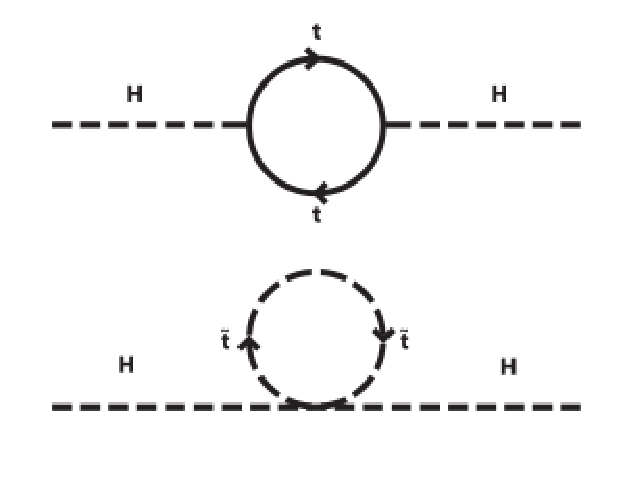
\includegraphics[width=0.5\textwidth]{Hierarchy.pdf}
 	\caption[Hierarchy Problem Loop Correction]{The loop corrections to the Higgs boson interacting with a top quark and its superpartner the top squark. This is a next-to-leading order (NLO) correction to the Higgs boson mass.}
 	\label{HiggsMass} 
\end{figure}

\subsection{Hierarchy Problem} 
The Higgs boson is a beautiful solution to electroweak symmetry breaking and gives a method for particles to acquire mass, see Sec. \ref{HiggsMechanism},  and was discovered to have a measured mass of $m_{H}=125.18\pm0.16$ GeV. This value though is not predictable with the SM and leads to some inconsistencies when you include loop corrections. Since the Higgs is strongly coupled to particles with large masses, the dominant loop correction is due to interactions with the $t$ quark. These higher order loop corrections to the Higgs mass, $m_H^2$, caused by the fermionic $t$ loop, see fig \ref{HiggsMass}, are,
\begin{equation} \label{HiggsDivergence}
\Delta m_{H}^{2}=-\frac{|\lambda_{t}|^{2}}{8\pi^{2}}\Lambda_{UV}^{2}+\cdot\cdot\cdot,
\end{equation}
where $\lambda_f$ is the vertex factor for the respective fermion and $\Lambda_{UV}$ is the ultraviolet momentum cutoff. The Higgs boson loop corrections are highly dependent on all virtual and real particles that couple to the Higgs field, we can see the corrections from Eqn. \ref{HiggsDivergence} from the $t$ quark will cause a large divergence. The quadratic divergence of the Higgs mass is only renormalizable with a fine tuning of the parameters $\lambda_f$ and $\Lambda_{UV}$. 

This means the only way for the SM to reconcile this unfortunate fact is to have a relatively lucky cancellation of very large numbers of order $10^{32}$ with equally small numbers. Fortunately, if we add the contribution of a bosonic partner of the fermion the Higgs loop corrections reduce to,
\begin{equation}
\Delta m_{H}^{2}=\frac{\lambda_{S}}{16\pi^{2}}[\Lambda_{UV}^{2} - 2m_{S}^{2}ln(\Lambda_{UV}/m_{S})+\cdot\cdot\cdot].
\label{HiggsRenormalization}
\end{equation}
With the introduction of a scalar partner to the $t$, there is a logarithmic divergence to the higgs boson mass and can be renormalized through the normal methods.

\subsection{Grand Unified Theory}

The SM is able to accurately describe three of the fundamental sources at typical energy scales, 1 to $10^{4}$ GeV, but idealy the forces would be able to merge into a single force at higher energies. This has not been directly observed, but many theories, such as supersymmetry (SUSY), predict its existence \cite{martin_supersymmetry_1997}.

At standard energies for particle physics experiments the difference in the strength of each force is quite noticeable. But it has been shown that in the SM the strengths of each force are dependent on the energy scale and it would be ideal that they converge to a single force at large energies, such as $10^{16}$ GeV. In fig. \ref{GUT}, we see the extrapolated energy scales of the forces in the SM shown as the dotted line. These unfortunately, do not meet at a single point to become one force, but if we include supersymmetry into the model we get a nice convergence between the forces \cite{martin_supersymmetry_1997}.

\begin{figure}
 	\centering
	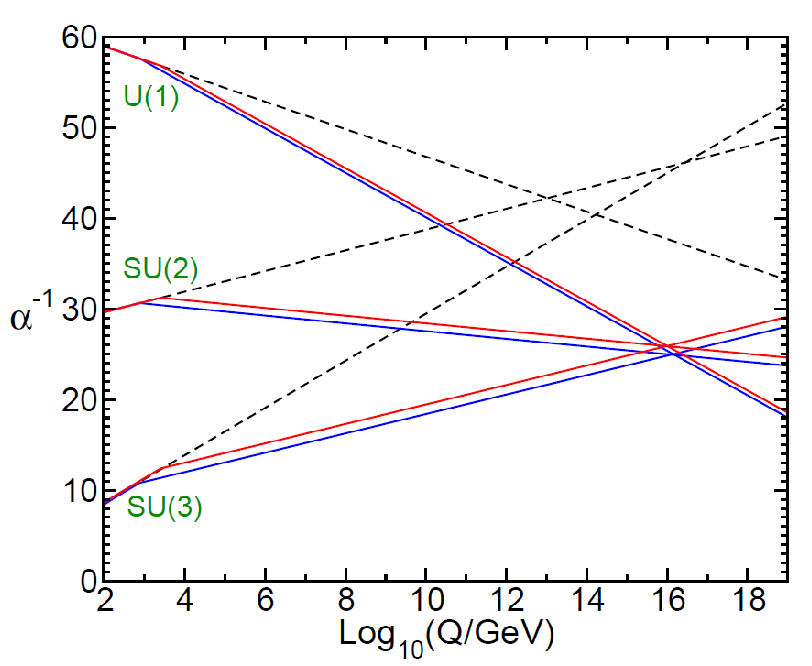
\includegraphics[width=0.5\textwidth]{GUTRenormalization.png}
 	\caption[GUT Force Energy Dependence]{The energy dependence of the inverse gauge couple of each force in the SM (dashed line) and the MSSM (solid lines). The MSSM gives two thresholds for the sparticle mass 750 GeV and 2.5 TeV.}
 	\label{GUT} 
\end{figure}

\section{Supersymmetry}

We have seen from the above three problems that there is still more to learn. Some of the features of the universe, such as; dark matter, the hierarchy problem, and a grand unified theory have not been explained. We saw from the Hierarchy problem that the addition of a bosonic partner to a fermion will allow for the loop corrections to be renormalizable without fine tuning. Fortunately, some theories have allowed for such a problem to be solved. Namely the theory of SUSY which essentially states that each particle in the SM has a superpartner that has only the spin changed, that every fermion has a bosonic partner that has all the same quantum numbers except the spins differ by $1/2$, and vice-versa.

\begin{figure}
 	\centering
	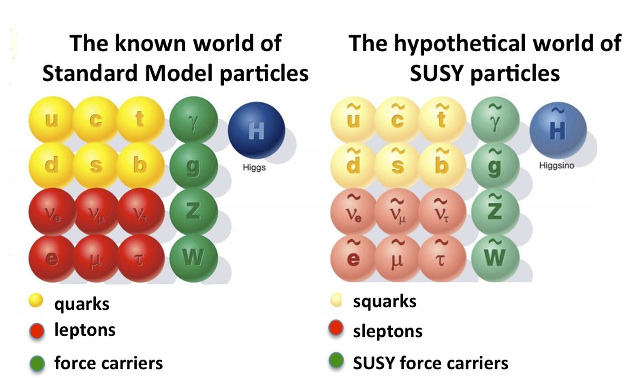
\includegraphics[width=0.75\textwidth]{SM-SUSY-diagram.jpg}
 	\caption[Supersymmetry and Standard Model Particles]{The corresponding SUSY particles which are partners to the SM particles.}
 	\label{SUSYParticles} 
\end{figure}

The partners to the fermions are denoted with a 's' in front of the name to notify that it is the scalar form of the particle and the partners to the bosons have an 'ino' attached at the end, such as photino, gluino, wino, and Higgsino. So for the partners to the fermionic particles in the standard model we have: sup $(\widetilde{u})$, sdown $(\widetilde{d})$, scharm $(\widetilde{c})$, sstrange $(\widetilde{s})$, stop $(\st)$, and sbottom $(\widetilde{b})$ for the squarks and selectron $(\widetilde{e})$, smuon $(\widetilde{\mu})$, and stau $(\widetilde{\tau})$ for the charged sleptons. The partners to the neutrinos, which are always left-handed if you neglect the minimal masses, are sneutrinos $(\widetilde{\nu}_e, \widetilde{\nu}_\mu, \widetilde{\nu}_\tau)$, where whe have one for each flavor of lepton, see Fig. \ref{SUSYParticles}. 

If the SUSY was unbroken the superpartners would have exactly the same properties as the SM pairs except their spin. This would cause a massless photino or a $m_{\widetilde{e}}=0.511$ keV selectron. These particles would certainly have been detected at this point, which leads us to think that SUSY is a broken symmetry where all the superpartners have a mass that is significantly higher than their SM partners. 

\subsection{Supermultiplets and Chirality}
\label{subsec:chiral}

A supermultiplets is any symmetry where the number of bosonic degrees of freedom and fermionic degrees of freedom are equal, $n_B=n_F$. The simplest  way to achieve this is to have a combination of a single Weyl fermion, which is a chiral representation of the fermion and has two spin helicity states, $n_F=2$, and two real scalars with each having $n_B=1$. It becomes convenient for the mathematics to combine the two real scalars into one complex scalar field. Now the combination of a complex scalar field and a Weyl fermion is known as a chiral supermultiplet. 

\subsection{Minimal Supersymmetric Standard Model}
\label{sec:MSSM}

We have discussed how the fermions transform under the rules of SUSY, but how do the scalar field mediators translate into this new framework. First, lets look at the Higgs boson. We know that there is not only one chiral supermultiplet. If there was only one in the electroweak gauge symmetry, with a Higgsino of spin-$1/2$, would not have the anomaly cancellation of the traces, $Tr[T^2_3Y]\neq0$ and $Tr[Y^3]\neq0$, where $T_3$ is the third component of weak isospin and $Y$ is the weak hypercharge. In the SM, the traces of these for the fermions are already satified. So we must include two chiral supermultiplets of the Higgsino, with $Y=\pm\frac{1}{2}$, see table \ref{ChiralSMultiplets}. 

It turns out that this is also necessary for the Higgsino to give mass to different particles in the SM. A Higgs boson with $Y=1/2$ has the Yukawa couplings that allow it to interact with the up-type quarks $(u, c, t)$. Only a Higgs boson with $Y=-1/2$ has the correct Yukawa couplings to interact with the down-type quarks $(d, s, b)$ and the charged leptons $(e, \mu, \tau)$.

\begin{table}
 	\centering
	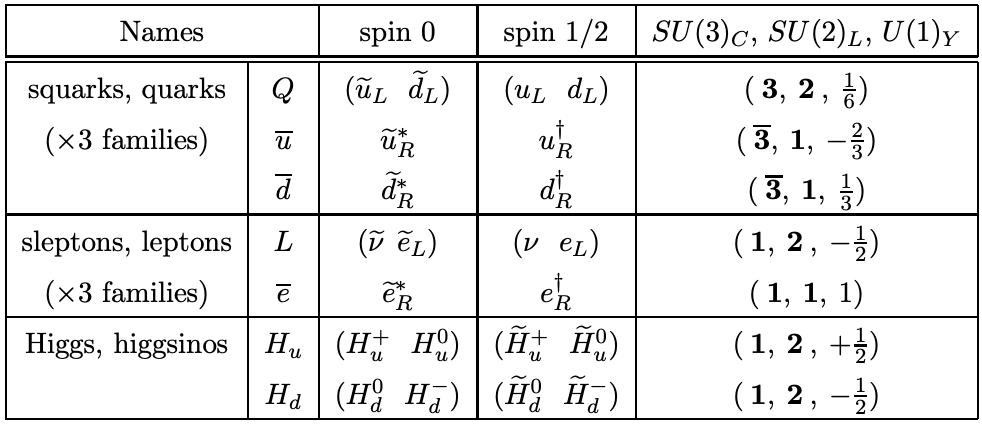
\includegraphics[width=0.7\textwidth]{ChiralSupermultiplets.png}
 	\caption[Chiral supermultiplets for fermions and bosons]{The chiral supermultiplets of the MSSM. Spin-0 fields are complex scalars and spin-$1/2$ fields are left-handed two component Weyl fermions \cite{martin_supersymmetry_1997}.}
 	\label{ChiralSMultiplets} 
\end{table}

\begin{table}
 	\centering
	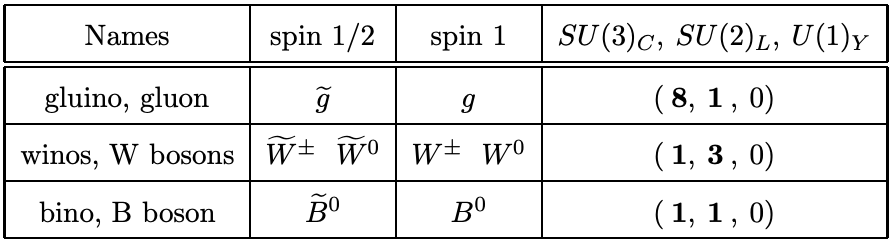
\includegraphics[width=0.7\textwidth]{GaugeSupermultiplets.png}
 	\caption[Chiral supermultiplets for gauge bosons]{The chiral supermultiplets of the MSSM \cite{martin_supersymmetry_1997}.}
 	\label{GaugeSMultiplets} 
\end{table}

The SM vector boson will also have a corresponding chiral supermultiplet. They have fermionic superpartners that are referred to as gauginos. For the $SU(3)_C$ color gauge interactions of QCD, which are a spin-$1/2$ color-octet, has a partner called a gluino $(\widetilde{g})$. The electroweak gauge theory $SU(2)_L\times U(1)_Y$ has the superpartners $\widetilde{\W}^+,\widetilde{\W}^0, \widetilde{\W}^-, \text{and } \widetilde{B}^0$ each with spin-$1/2$, called winos and bino, see table \ref{GaugeSMultiplets}. The gaugino mixtures of $\widetilde{\W}^0$ and $\widetilde{B}^0$ give the corresponding zino $(\widetilde{Z}^0)$ and photino $(\widetilde{\gamma})$. The chiral supermultiplets shown in table \ref{ChiralSMultiplets} and \ref{GaugeSMultiplets} give the particles of the Minimal Supersymmetric Standard Model (MSSM). 

The five higgsinos and electroweak gauginos mix with each other to because of electroweak symmetry breaking \cite{martin_supersymmetry_1997}. The neutral higgsinos $(\widetilde{H}_u^0 \text{ and } \widetilde{H}_d^0)$ and neutral gauginos $(\widetilde{B} \text{ and } \widetilde{W}^0)$ mix into four mass eigenstates, which are called neutralinos, $\neutralino, \widetilde{\chi}^0_2, \widetilde{\chi}^0_3, \text{ and }\widetilde{\chi}^0_4$. The charged higgsinos $(\widetilde{H}_u^+ \text{ and } \widetilde{H}_d^-)$ and charged gauginos $(\widetilde{W}^+\text{ and } \widetilde{W}^-)$ can mix into two mass eigenstates with charge $\pm1$ called charginos,  $\widetilde{\chi}^\pm_1 \text{ and } \widetilde{\chi}^\pm_2$. 

\subsection{R Parity}
\label{subsec:rparity}

$R$-parity or matter parity is the multiplicatively conserved quantum number defined as, 
\begin{equation} \label{RParity}
P_R=(-1)^{3(B-L)+2s}, 
\end{equation}
where $B$ is the baryon number, $L$ is the lepton number, and $s$ is the spin of the particle. From this we can find the $R$-parity of all the particles in the SM and MSSM. The definition of $R$-parity is quite useful because all the particles of the SM have an $R$-partity of $P_R=+1$, while all of the squarks, sleptons, gauginos, and higgsinos have $P_R=-1$.

$R$-parity is thought to be exactly conserved in SUSY, where there is no mixing between particles $(P_R=+1)$ and sparticles $(P_R=-1)$. This leads to three important consequences:
\begin{itemize}
	 \item The lightest sparticle that has $P_R=-1$ is called the "lightest supersymmetric particle" or LSP, which must be absolutely stable. If it is electrically neutral, it is a possible non-baryonic dark matter candidate.
	 \item Every sparticle, other than the LSP, must eventually decay into an odd number of LSPs.
	 \item For collider experiments, sparticles will only be produced in even numbers.
\end{itemize}
 We are going to be investigating a MSSM that conserves $R$-parity. This is quite well motivated by the possiblilty of a dark matter candidate. 

\subsection{Mass Spectrums}

\begin{figure}
\centering
	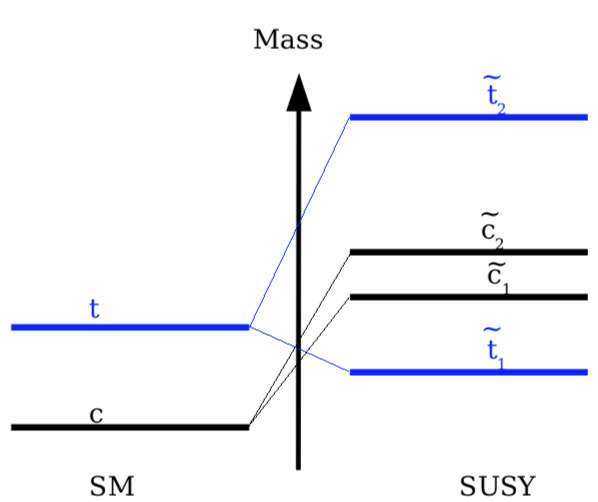
\includegraphics[width=0.5\textwidth]{TopSquarkMass.png}
 	\caption[Top squark mass hierarchy]{On the right we have the arbitrary masses of the top and charm quarks. The left and right handed states mix into two mass eigenstates. It is possible that the top squark will have the smallest mass of the squarks.}
 	\label{StopMass} 
\end{figure}

The third family of squarks and sleptons should have quite different masses compared to their first- and second-family counterparts, which is caused by the large Yukawa $(y_t, y_b, y_\tau)$ and soft $(a_t, a_b, a_\tau)$ couplings, which are holomorphic parameters proportional to the Yukawa couplings. This causes significant mixing between the chiral superpartners $(\widetilde{t}_L, \widetilde{t}_R), (\widetilde{b}_L. \widetilde{b}_R)\text{, and } (\widetilde{\tau}_L, \widetilde{\tau}_R)$. We will concentrate on how the mass of the top squark, \st{} evolves in the MSSM. Given many contributions to the top squark mass such as; squared-mass terms, 4-vertex interactions terms with the up-type Higgs, the 3-vertex interactions with the down-type Higgs, and scalar potential couplings. We have a square-mass matrix for the top squarks, 
\begin{equation}
\mathcal{L}_{\text{stop masses}}=-
\begin{bmatrix}
\st^*_L & \st^*_R \\
\end{bmatrix}
\boldsymbol{m_{\st}^2}
\begin{bmatrix}
\st_L \\
\st_R \\
\end{bmatrix}
\end{equation}
where 
\begin{equation}
\boldsymbol{m_{\st}^2}=
\begin{bmatrix}
m_{Q_3}^2+m_t^2+(\frac{1}{2}-\frac{2}{3}sin^2\theta_W)cos(2\beta)m_Z^2 & v(a_t^*sin\beta-\mu y_tcos\beta) \\
v(a_tsin\beta-\mu^*y_tcos\beta) & m^2_{\overline{u}_3} +m_t^2+(\frac{2}{3}sin^2\theta_W)cos(2\beta)m^2_Z \\ 
\end{bmatrix}.
\end{equation}

This is a hermitian matrix and can be diagonalized to give eigenstates $\st_1$ and $\st_2$ which are linear combinations of the left and right-handed \st, see fig. \ref{StopMass}. Now we get the eigenvalues for the mass states as $m_{\st_1}^2<m_{\st_2}^2$. From this models predict that the $\st_1$ is the lightest squark \cite{martin_supersymmetry_1997}. 

\subsection{Supersymmetry Searches}
The SM of particle physics has been a powerful model for predicting interactions between quarks, leptons, and force carriers, with an accurate prediction for precision measurements, but has some faults such as, the Hierarchy problem, dark matter, and a Grand Unified Theory. We have seen that including SUSY can allow for possible solutions, such as: a dark matter candidate as the LSP, bosonic-fermionic loop corrections for the Higgs boson mass, and a unification of the fundamental forces at large energies. Then once investigating the theory of SUSY we were able to determine that the top squark could be the lightest squark, which allows us to develop multiple searches for this proposed theory. 

\section{Current SUSY Results}\label{CurrentResults}

Here we see the most current results from searches for the top squark. These have been completed with data from the first part of Run 2 with $35.9 \text{ fb}^{-1}$. This analysis was completed with the most up-to-date identification methods for particles in the SM. From this Analysis, all 104 search region bins, as well as the corresponding single-lepton control region bins, the $\gamma+$jets control region bins and the QCD control regions, are fit simultaneously in order to evaluate the cross section excluded at 95\% confidence level for each signal benchmark point. 

The easiest way to think about the plots shown in \ref{T2ttANLimits}, \ref{T2bWANLimits}, \ref{T2tbANLimits}, \ref{T2fbdANLimits}, \ref{T2bWCANLimits}, is that there is a calculated limit for each mass point. The $x$-axis is the possible mass range for the \st, $m_{\st}$ and the y-axis is the possible range for the \neutralino, $m_{\neutralino}$. Each point in this 2D space has a color representation for the value of the upper limit on the cross section at a confidence level of 95\%. 

With the comprehensive analysis that was performed in 2016, we have various limits on the multiple decay modes of the \st{} which will be covered completely in Section \ref{ch:Search}. The comprehensive limits on the \st{} mass range from values of 550 to 1.1 \TeV{} for all of the all-hadronic decay modes. The CMS Collaboration has also combined the limits from the separate analyses which concentrate on the 1-lep, 2-lep, MT2, and HT missing analyses. The conbination of these has shown that we can set limits on the \st{} mass range for masses of 800 to 1100 \GeV. 

\begin{figure}
\centering
	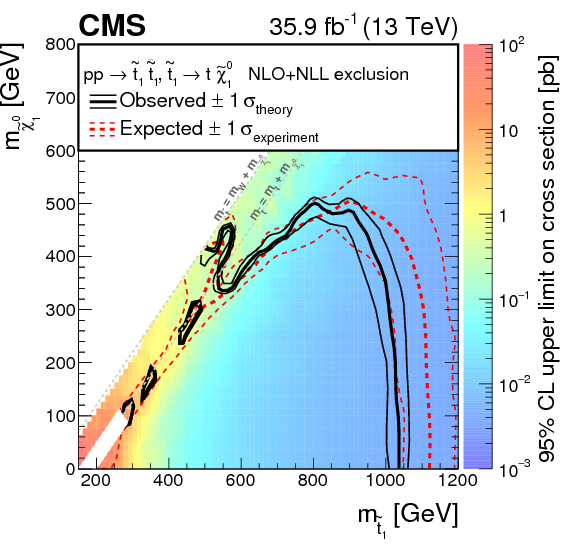
\includegraphics[width=0.50\textwidth]{T2tt_AN16.png}
 	\caption[T2tt Limits]{Limits for the mass parameter space for T2tt decays. With a current limit of 1.1 \TeV{} for a minimal neutralino mass.}
 	\label{T2ttANLimits} 
\end{figure}

\begin{figure}
\centering
	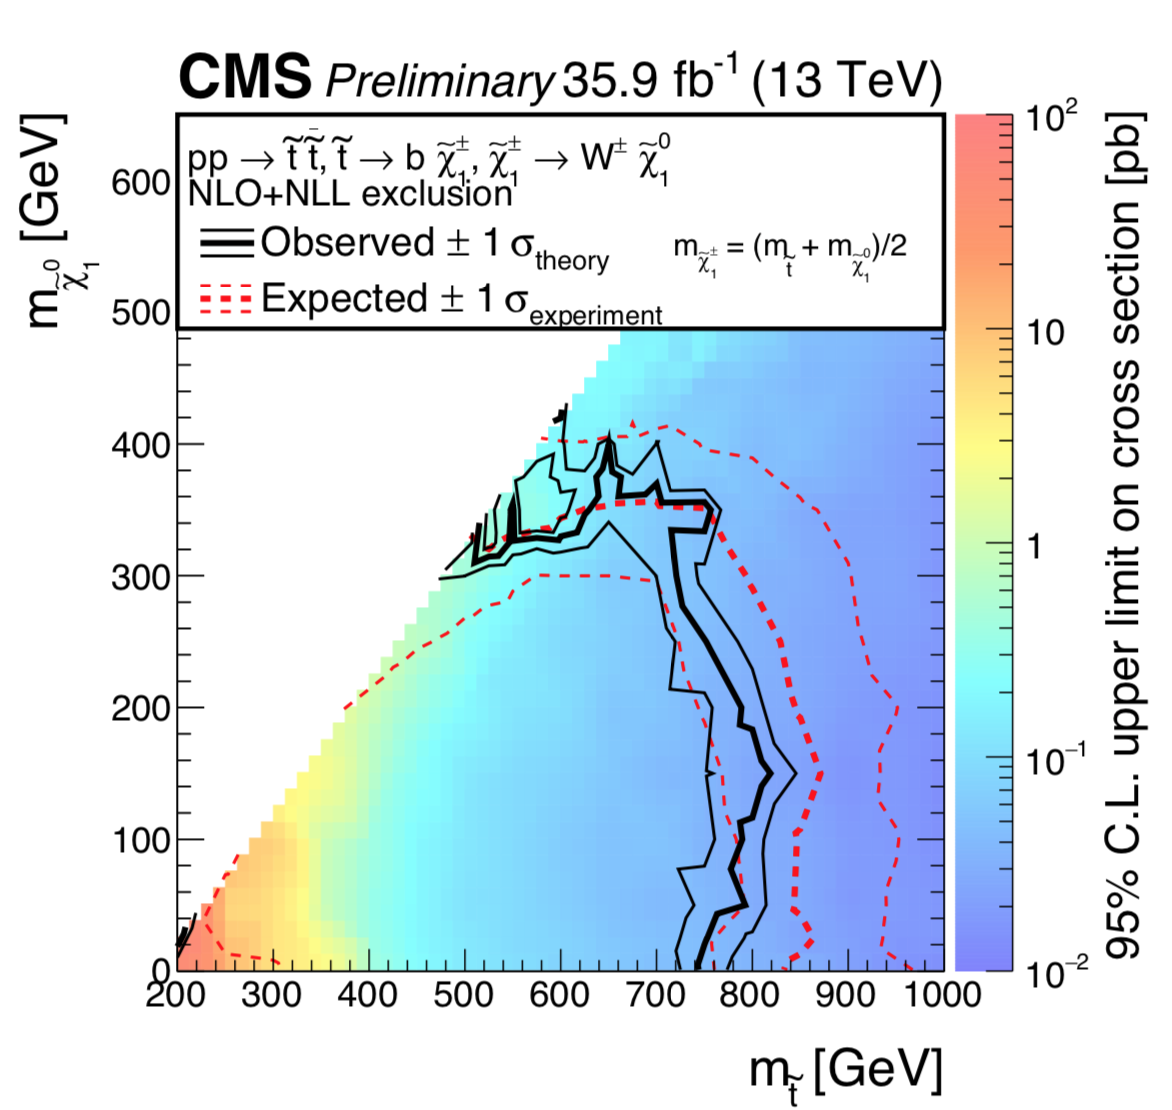
\includegraphics[width=0.50\textwidth]{T2bW_AN16.png}
 	\caption[T2bW Limits]{Limits for the mass parameter space for T2bW decays. With a current limit of 750 \GeV{} for a minimal neutralino mass.}
 	\label{T2bWANLimits} 
\end{figure}

\begin{figure}
\centering
	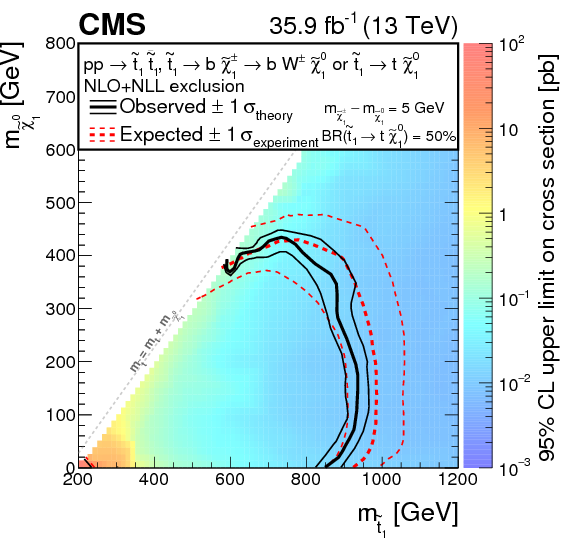
\includegraphics[width=0.50\textwidth]{T2tb_AN16.png}
 	\caption[T2tb Limits]{Limits for the mass parameter space for T2tb decays. With a current limit of 850 \GeV{} for a minimal neutralino mass.}
 	\label{T2tbANLimits} 
\end{figure}

\begin{figure}
\centering
	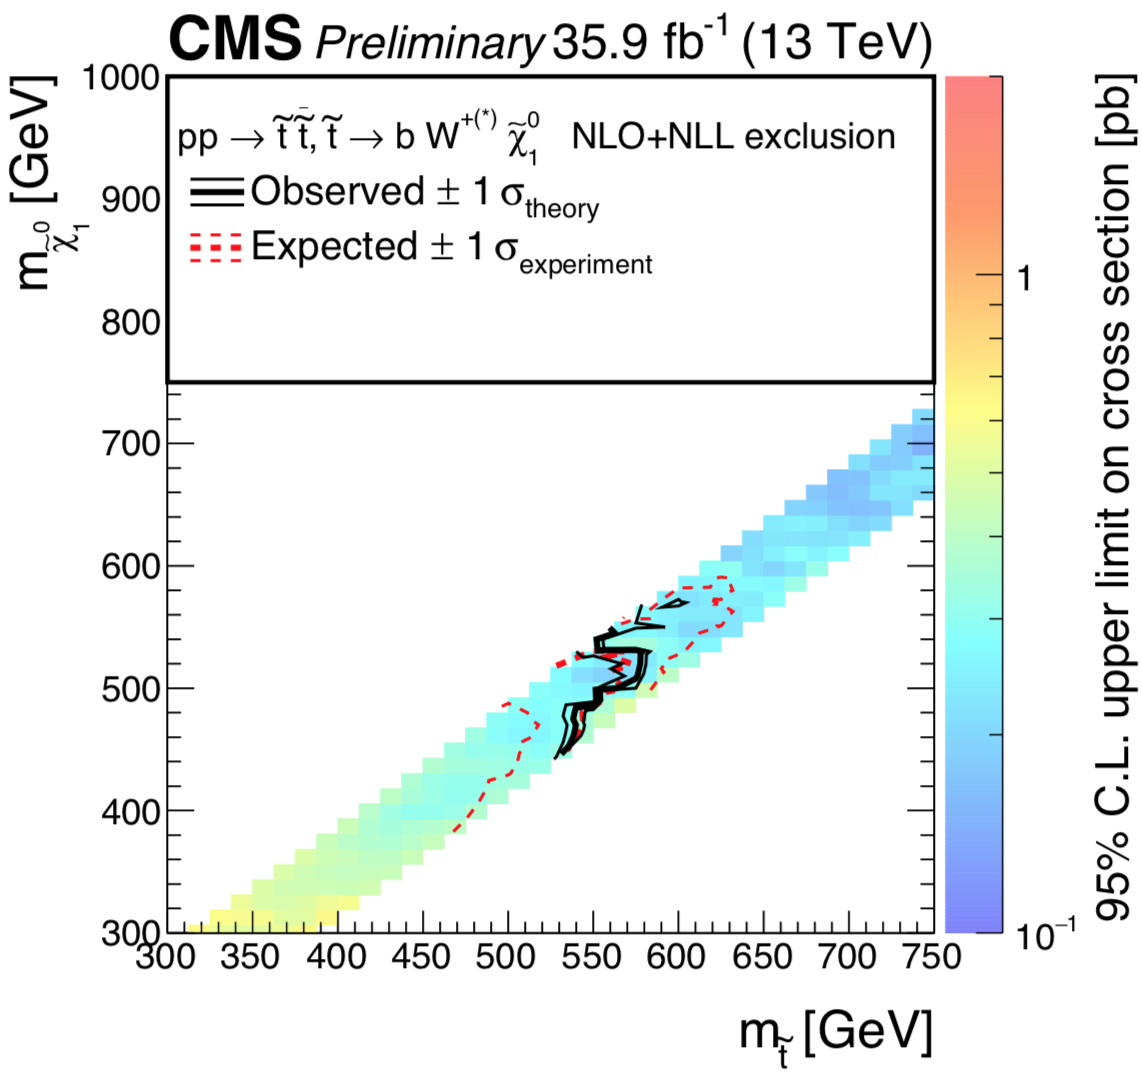
\includegraphics[width=0.50\textwidth]{T2fbd_AN16.png}
 	\caption[T2fbd Limits]{Limits for the mass parameter space for T2fbd decays. Which has a range of 550 \GeV{} for a \neutralino{} mass of approx. 500 \GeV.}
 	\label{T2fbdANLimits} 
\end{figure}

\begin{figure}
\centering
	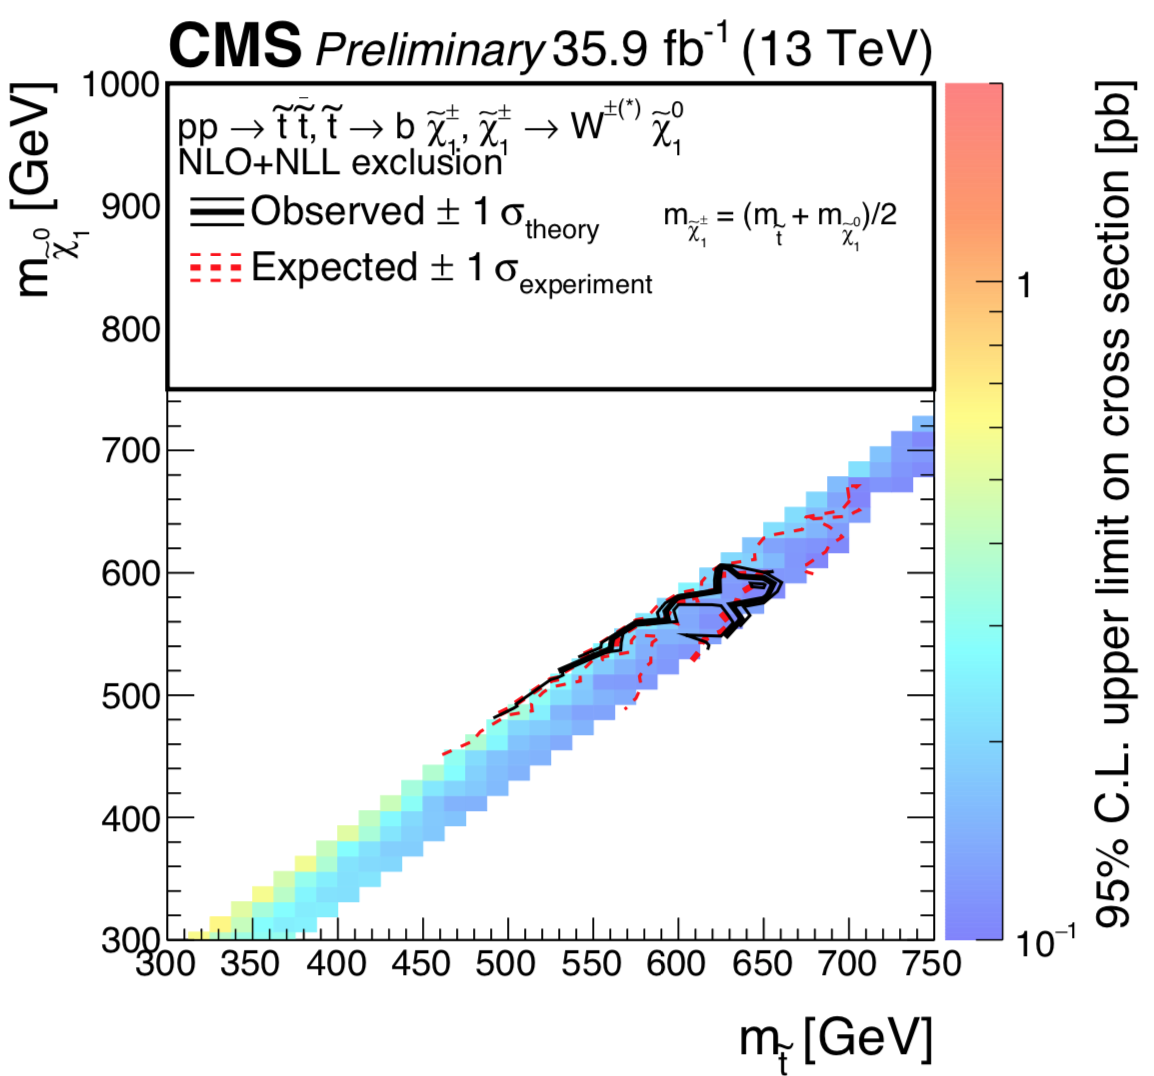
\includegraphics[width=0.50\textwidth]{T2bWC_AN16.png}
 	\caption[T2bWC Limits]{Limits for the mass parameter space for T2bWC decays. Which has a range of 550 to 675 \GeV{} for a \neutralino{} mass of 600 \GeV.}
 	\label{T2bWCANLimits} 
\end{figure}

\begin{figure}
\centering
	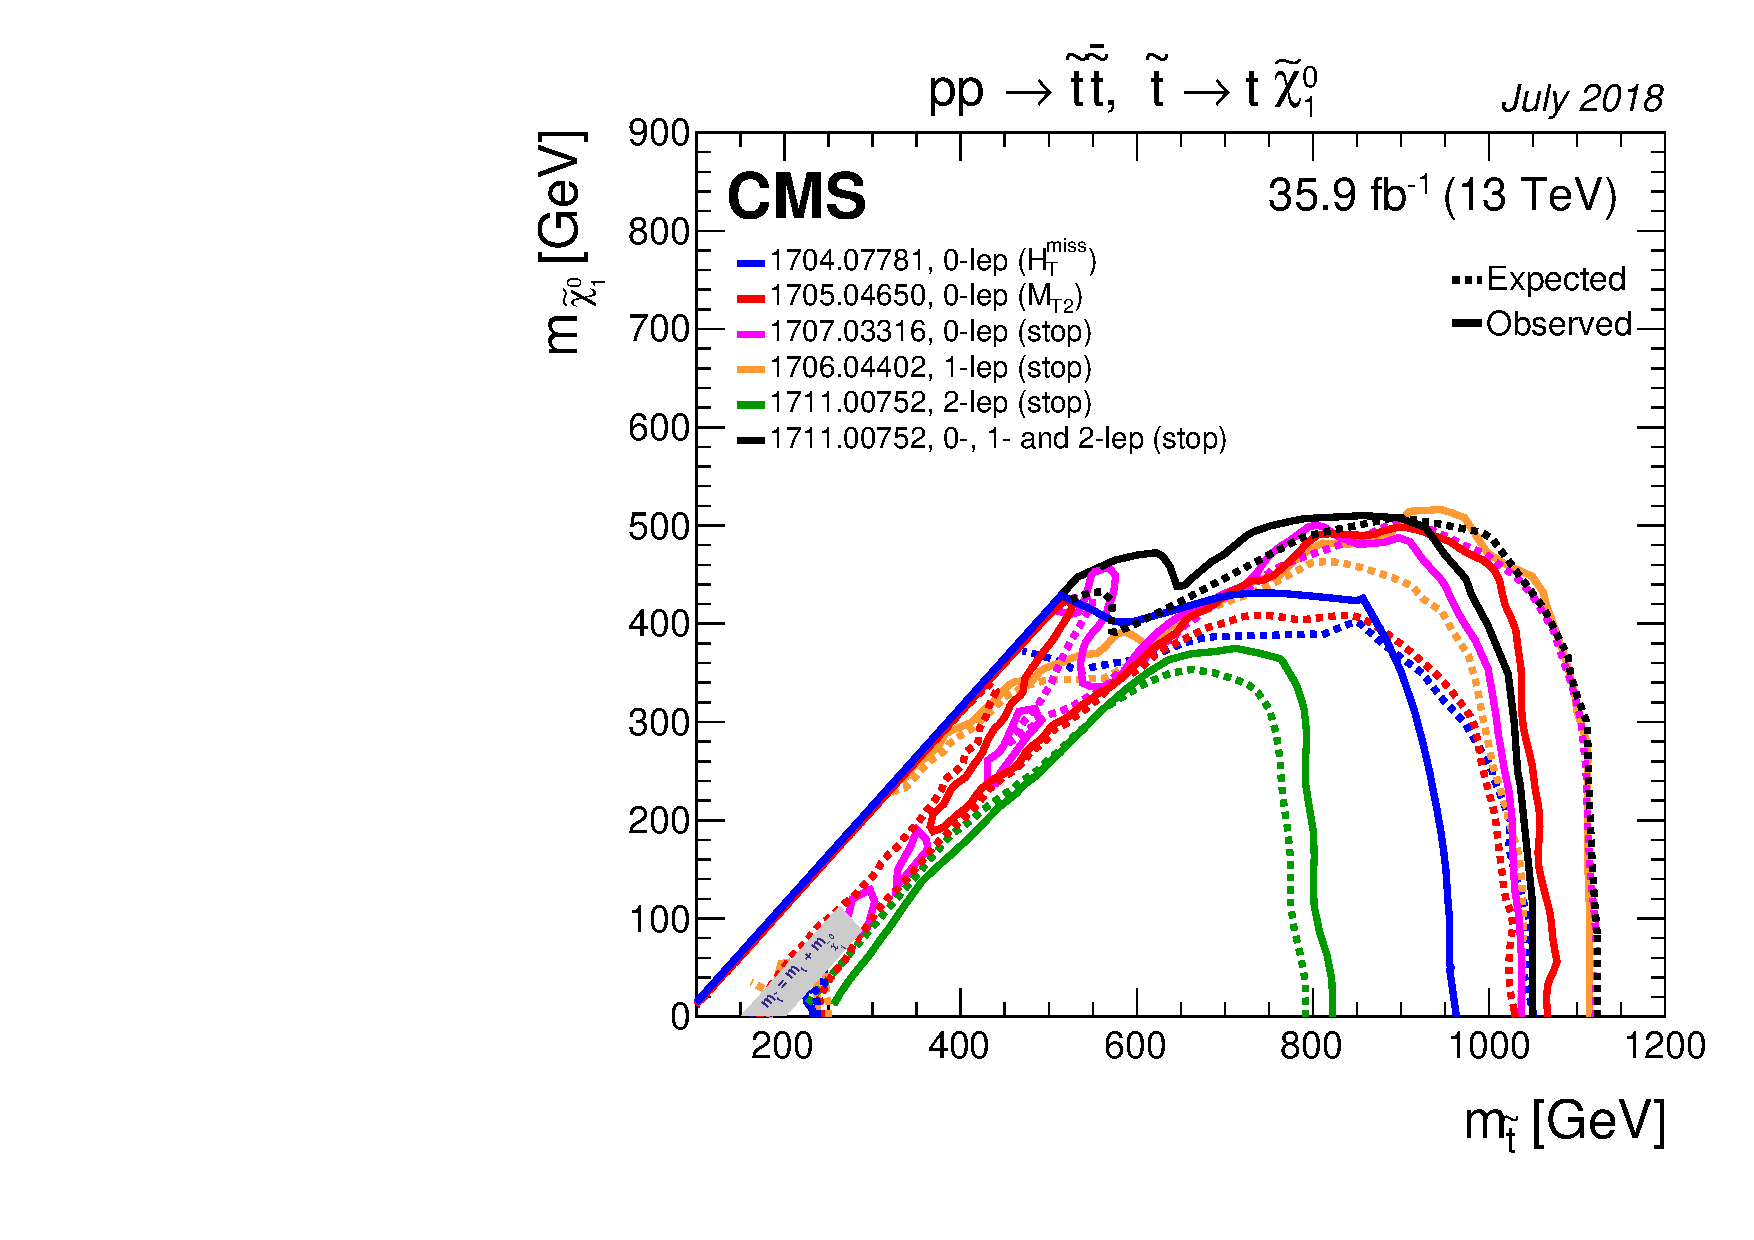
\includegraphics[width=0.50\textwidth]{T2tt_limits_summary_cms.pdf}
 	\caption[T2tt Limits for all decay modes]{Limits for the mass parameter space for T2tt decays using results from all the analysis in CMS. With a current limit of 1.1 \TeV{} for a minimal neutralino mass.}
 	\label{T2ttCMSAll} 
\end{figure}

From the above plots, \ref{T2ttANLimits}, \ref{T2bWANLimits}, \ref{T2tbANLimits}, \ref{T2fbdANLimits}, \ref{T2bWCANLimits}, and \ref{T2ttCMSAll}, we know that we are able to exclude a large mass range for the \st{} and \neutralino{}. Since this is one for a luminosity of 36.8 \fb, we can expect improved limits with all of the data from Run 2, which is 137 \fb. The new version of the analysis also has a redesigned search region to allow for more sensitive results, while also impoving various object definitions.

\section{Improved Methods}
Search have been performed on the 36.8 \fb{} dataset from CMS. We have been able to exclude a mass range of 800 to 1100 \GeV{} from the previous analysis. With the included luminosity and updated analysis methods we expect to significantly improve these results. 
